\section{问题三：算力约束下的多维资源联合优化与结构性转移}
\label{sec:q3}

\subsection{优化模型}

以问题二选定的广义标度律为目标函数，在总算力预算下最小化验证损失：

\begin{equation}
\min_{N,D,Q,p}\ \widehat{L}(N,D,Q,p)=E+AN^{-\alpha}+B\left[DQ^{\kappa}h(p)\right]^{-\beta}
\end{equation}

\begin{equation}
\text{s.t.}\quad
\underbrace{6ND}_{C_{\mathrm{train}}}+\underbrace{\eta ND\ell}_{C_{\mathrm{attn}}}+\underbrace{D\left[g(Q)-g(Q_0)\right]_+}_{C_Q}\le C,
\qquad p_i\ge0,\ \sum_i p_i=1 .
\label{eq:q3_con}
\end{equation}

按题面，$\ell$ 为外生情景变量，$p$ 固定为问题一得到的优选配比（理由见\ref{sec:q3_fixp}节），$Q_0$ 取 0.5。三类质量成本函数为

\begin{table}[htbp]
\centering
\caption{题给三类质量成本函数}
\label{tab:q3_cost}
\small
\begin{tabular}{l|l|l|l}
\toprule
\textbf{类型} & \textbf{形式} & \textbf{参数} & \textbf{$Q=1$ 时的单位成本} \\
\midrule
指数型 & $g(Q)=\gamma e^{\lambda Q}$ & $\gamma=10^{7},\ \lambda=6.0$ & $4.03\times10^{9}$ \\
幂函数型 & $g(Q)=\gamma Q^{\lambda}$ & $\gamma=5\times10^{9},\ \lambda=4.0$ & $5.00\times10^{9}$ \\
对数渐进型 & $g(Q)=\gamma\ln(1+\lambda Q)$ & $\gamma=2\times10^{9},\ \lambda=10.0$ & $4.80\times10^{9}$ \\
\bottomrule
\end{tabular}
\end{table}

三者在 $Q=1$ 处的量级相近（$4\sim5\times10^9$），因而比较的是\textbf{曲线形状}而非绝对成本水平，这正是题面希望考察的。

\subsection{约束化简与解析参照}

\subsubsection{消去 $D$}

三个成本项共用同一个 $D$，约束可整理为

\begin{equation}
D\left\{(6+\eta\ell)N+\left[g(Q)-g(Q_0)\right]_+\right\}\le C .
\label{eq:q3_budget}
\end{equation}

由于 $\partial L/\partial D<0$ 恒成立，且题面未给出数据量上限，最优点处约束必取等号，于是

\begin{equation}
D^\ast(N,Q)=\frac{C}{(6+\eta\ell)N+\left[g(Q)-g(Q_0)\right]_+}.
\label{eq:q3_D}
\end{equation}

代入目标函数后，问题降为 $(\log N,Q)$ 上的二维无约束优化，$D$ 由式\eqref{eq:q3_D}精确回代。这一化简的两个前提（损失对 $D$ 单调、无额外 $D$ 上限）在\ref{sec:q3_check}节逐点核验。

\subsubsection{固定 $Q$ 时的解析参照}

当 $Q$ 固定且无质量开销时，$\partial L/\partial N=0$ 给出闭式解

\begin{equation}
N^\ast=\left[\frac{\alpha A\left(Q^{\kappa}C/a\right)^{\beta}}{\beta B}\right]^{\frac{1}{\alpha+\beta}},
\qquad a=6+\eta\ell,
\label{eq:q3_analytic}
\end{equation}

回代得 $D^\ast=C/(aN^\ast)$。该式用于校验数值搜索的正确性。

\subsection{求解方法}

\subsubsection{为什么不用常规二维优化}

本文发现该损失面对 $N$ 极为平坦：在最优解附近，$N$ 变化近两倍而损失变化不足 $10^{-4}$ nat。这种情形下 Nelder--Mead 等直接二维搜索会过早收敛。实测把二者对比：解析最优为 $N^\ast=4.46\times10^8$，而 Nelder--Mead 返回 $7.16\times10^8$，相对偏差 60\%，尽管损失差仅 $9.5\times10^{-6}$。

因此本文采用\textbf{外层 $Q$ 网格 + 内层对 $\log N$ 有界黄金分割极小化 + 坐标下降细化}的策略：内层一维搜索用 \texttt{minimize\_scalar(method='bounded')}，对单峰平坦函数是稳健的；外层在 $Q\in[Q_0,1]$ 上先取 200 点网格，再在最优邻域内加密。修正后数值解与解析解在全部 15 个 $(C,\ell)$ 组合上的相对偏差均小于 $1.1\times10^{-6}$（表~\ref{tab:q3_analytic}）。

\begin{table}[htbp]
\centering
\caption{解析参照与数值搜索的一致性（固定 $Q=Q_0$，指数型成本）}
\label{tab:q3_analytic}
\small
\begin{tabular}{r|r|r|r|r}
\toprule
$C$ (FLOPs) & $\ell$ & $N^\ast$ 解析 & $N^\ast$ 数值 & 相对偏差 \\
\midrule
$10^{19}$ & 2\,048 & $2.1348\times10^{7}$ & $2.1348\times10^{7}$ & $9.5\times10^{-7}$ \\
$10^{19}$ & 8\,192 & $1.9722\times10^{7}$ & $1.9722\times10^{7}$ & $2.0\times10^{-7}$ \\
$10^{19}$ & 131\,072 & $1.0298\times10^{7}$ & $1.0298\times10^{7}$ & $6.3\times10^{-10}$ \\
$10^{22}$ & 8\,192 & $4.4620\times10^{8}$ & $4.4620\times10^{8}$ & $6.7\times10^{-7}$ \\
$10^{24}$ & 8\,192 & $3.5692\times10^{9}$ & $3.5692\times10^{9}$ & $8.4\times10^{-7}$ \\
$10^{24}$ & 131\,072 & $1.8636\times10^{9}$ & $1.8636\times10^{9}$ & $1.0\times10^{-6}$ \\
\bottomrule
\end{tabular}
\end{table}

\subsubsection{固定配比的理由}
\label{sec:q3_fixp}

题面允许 $p$ 作为联立决策变量，也允许由前两问确定。本文选择后者，理由有三：（1）问题一已证明配比效应可以跨参数规模迁移（60M 检验集 Spearman 达 0.706），固定优配比是合理的近似；（2）在广义标度律中，配比通过 $h(p)$ 以\textbf{可分离因子}的形式进入，若不引入与配比相关的成本或供给约束，最优 $p$ 将与预算无关，强行做``配比随预算转移''的结论会是伪发现；（3）$\omega$ 本身不可辨识（\ref{sec:q2_quality}节），联立优化 $p$ 会把这一不确定性放大到配置结论上。本文在\ref{sec:q3_sens}节对 $\omega$ 做了情景敏感性分析。

\subsection{优化结果}

\subsubsection{三档预算与三类成本}

表~\ref{tab:q3_main} 给出 $\ell=8192$ 时的主结果，图~\ref{fig:q3_path} 与图~\ref{fig:q3_share} 给出连续变化。

\begin{table}[htbp]
\centering
\caption{最优配置（$\ell=8192$，$Q_0=0.5$，$\kappa=1.052$）}
\label{tab:q3_main}
\small
\begin{tabular}{r|l|r|r|r|r|r|r}
\toprule
$C$ (FLOPs) & \textbf{成本函数} & \textbf{$N^\ast$ (B)} & \textbf{$D^\ast$ (B)} & \textbf{$Q^\ast$} & \textbf{质量份额} & \textbf{注意力份额} & \textbf{预测损失} \\
\midrule
\multirow{3}{*}{$10^{19}$} & 指数型 & 0.0197 & 66.4 & 0.500 & 0\% & 21.4\% & 1.69239 \\
                            & 幂函数型 & 0.0197 & 66.4 & 0.500 & 0\% & 21.4\% & 1.69239 \\
                            & 对数渐进型 & 0.0197 & 66.4 & 0.500 & 0\% & 21.4\% & 1.69239 \\
\midrule
\multirow{3}{*}{$10^{22}$} & 指数型 & 0.716 & 1\,497 & \textbf{0.826} & \textbf{18.2\%} & 17.5\% & 1.69066 \\
                            & 幂函数型 & 0.738 & 1\,384 & \textbf{0.785} & \textbf{22.0\%} & 16.7\% & 1.69067 \\
                            & 对数渐进型 & 0.771 & 1\,408 & \textbf{1.000} & 17.1\% & 17.8\% & 1.69063 \\
\midrule
\multirow{3}{*}{$10^{24}$} & 指数型 & 5.49 & 21\,842 & \textbf{1.000} & 8.4\% & 19.7\% & 1.69020 \\
                            & 幂函数型 & 5.60 & 21\,073 & \textbf{1.000} & 9.9\% & 19.3\% & 1.69020 \\
                            & 对数渐进型 & 5.14 & 24\,708 & \textbf{1.000} & 3.0\% & 20.8\% & 1.69020 \\
\bottomrule
\end{tabular}
\end{table}

\begin{figure}[htbp]
\centering
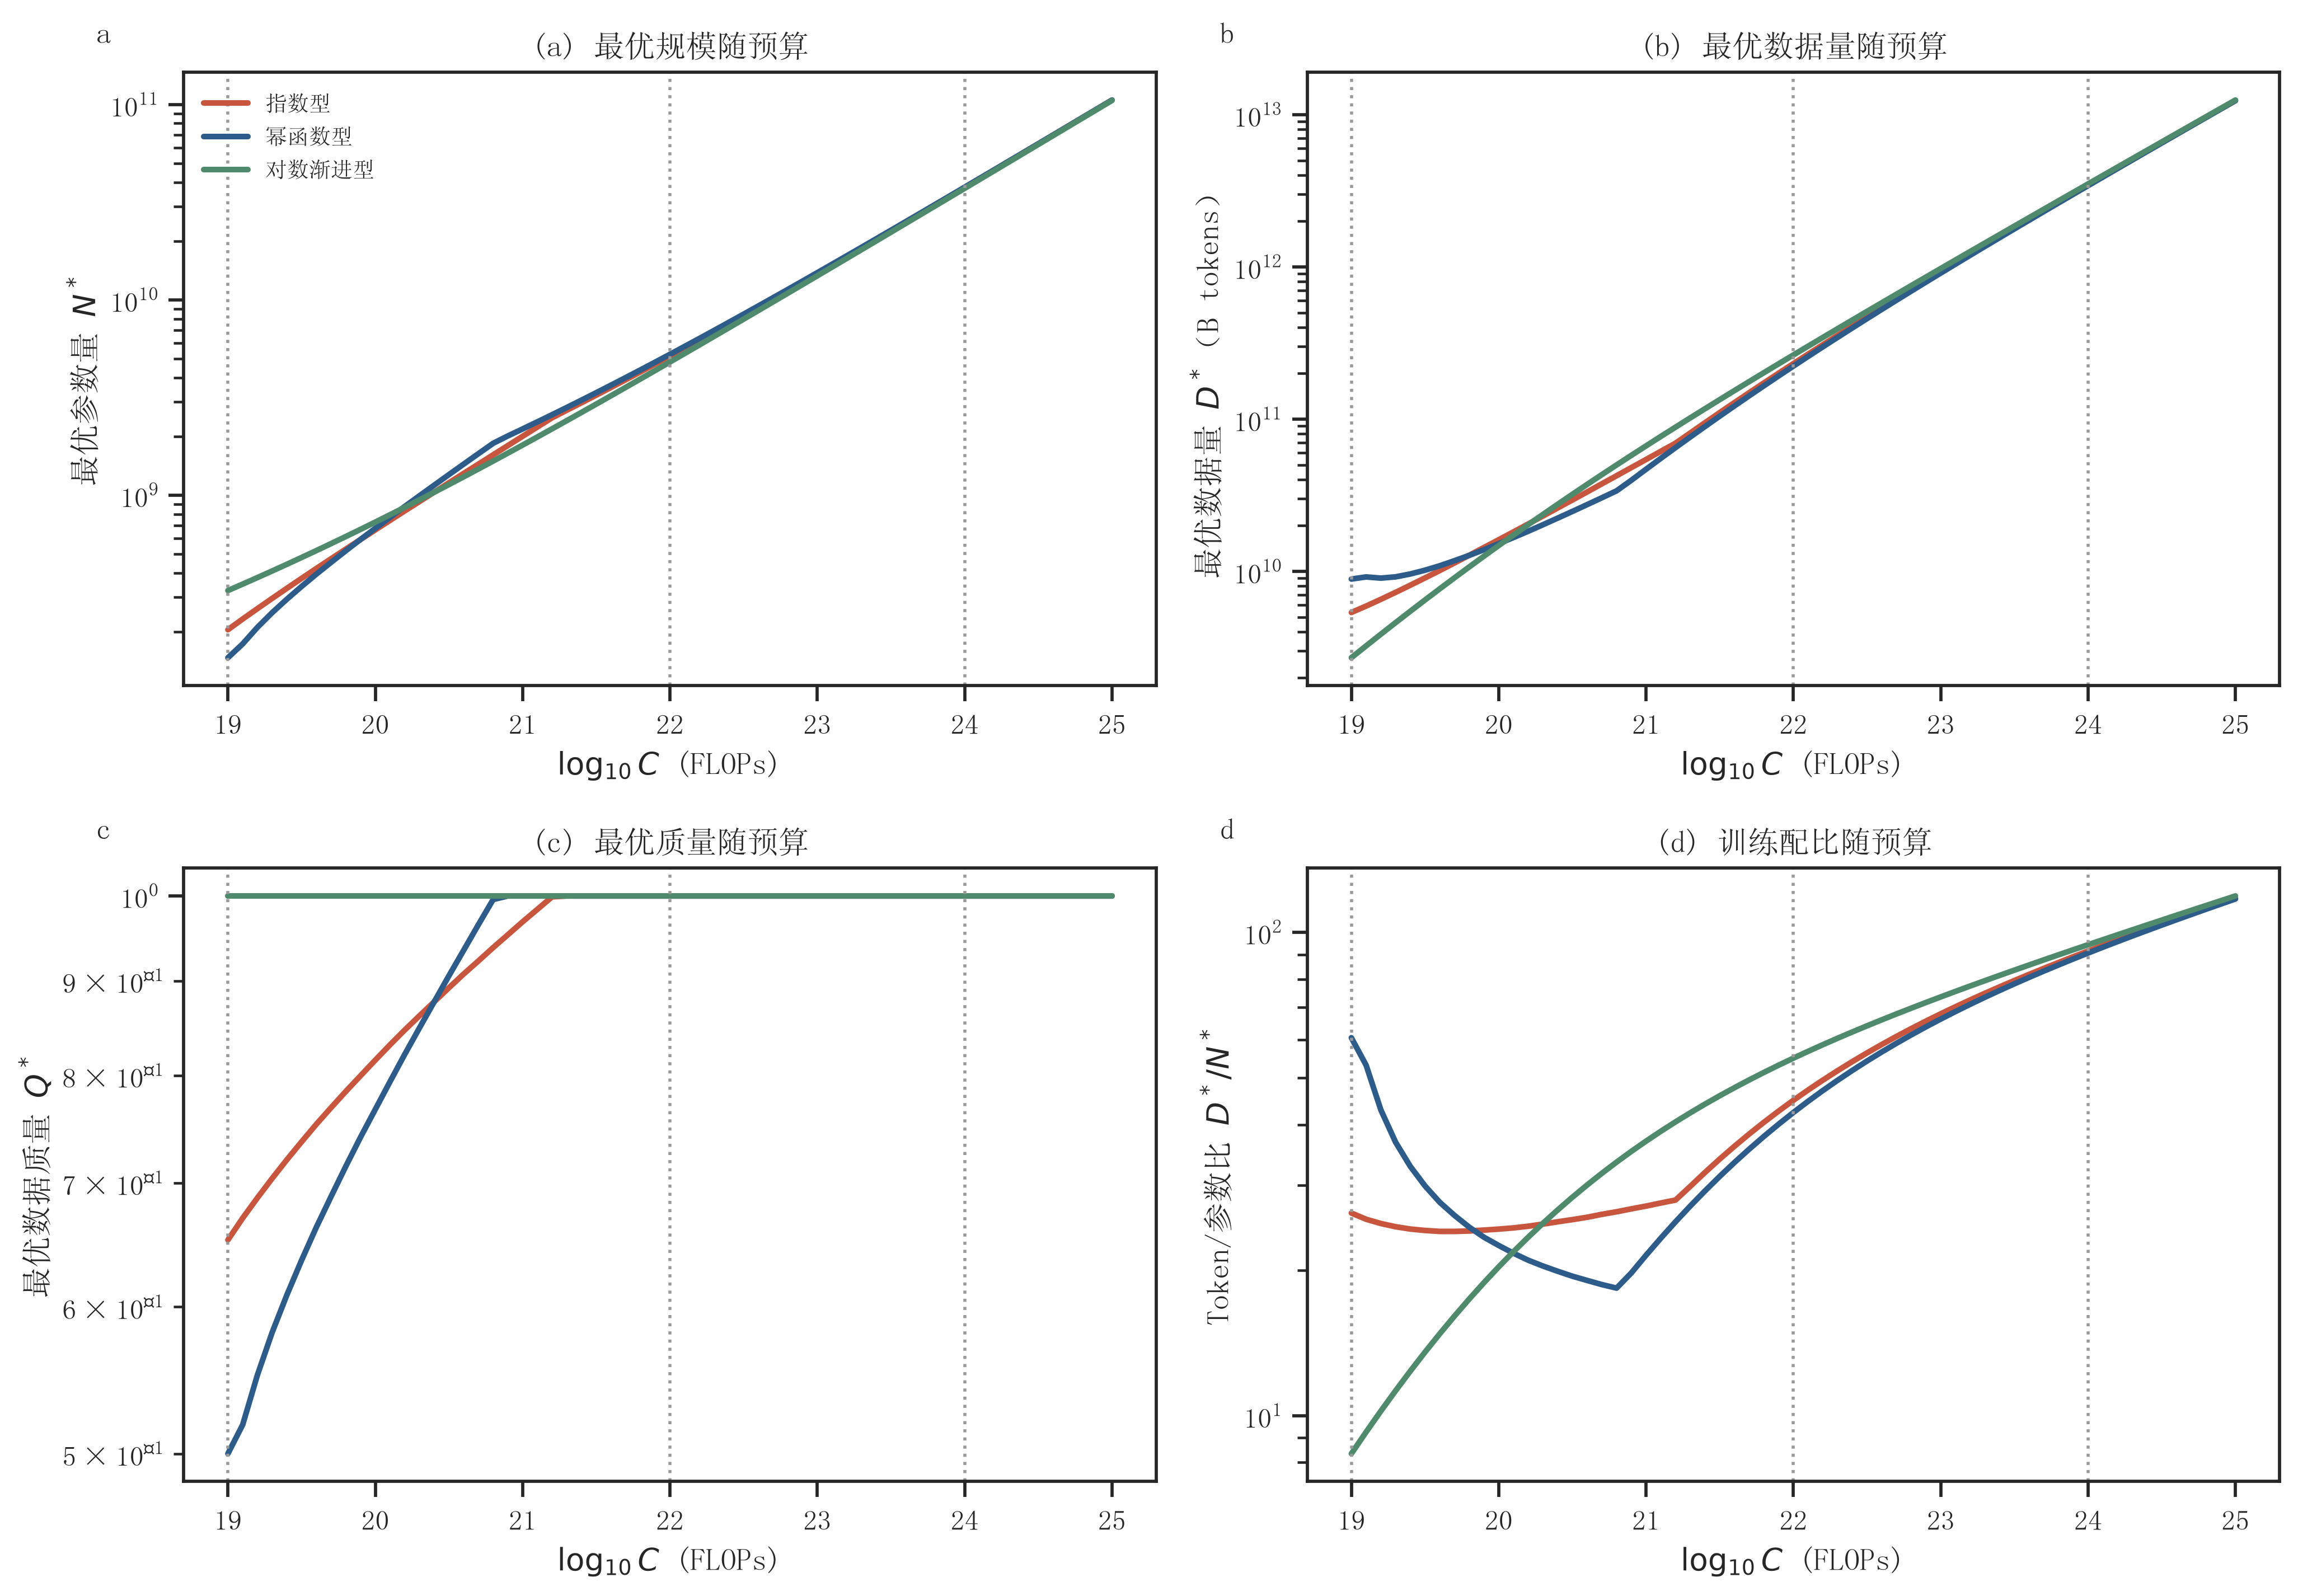
\includegraphics[width=0.95\textwidth]{figures/fig_q3_budget_paths.png}
\caption{最优配置随预算的连续变化}
\label{fig:q3_path}
\end{figure}

\begin{figure}[htbp]
\centering
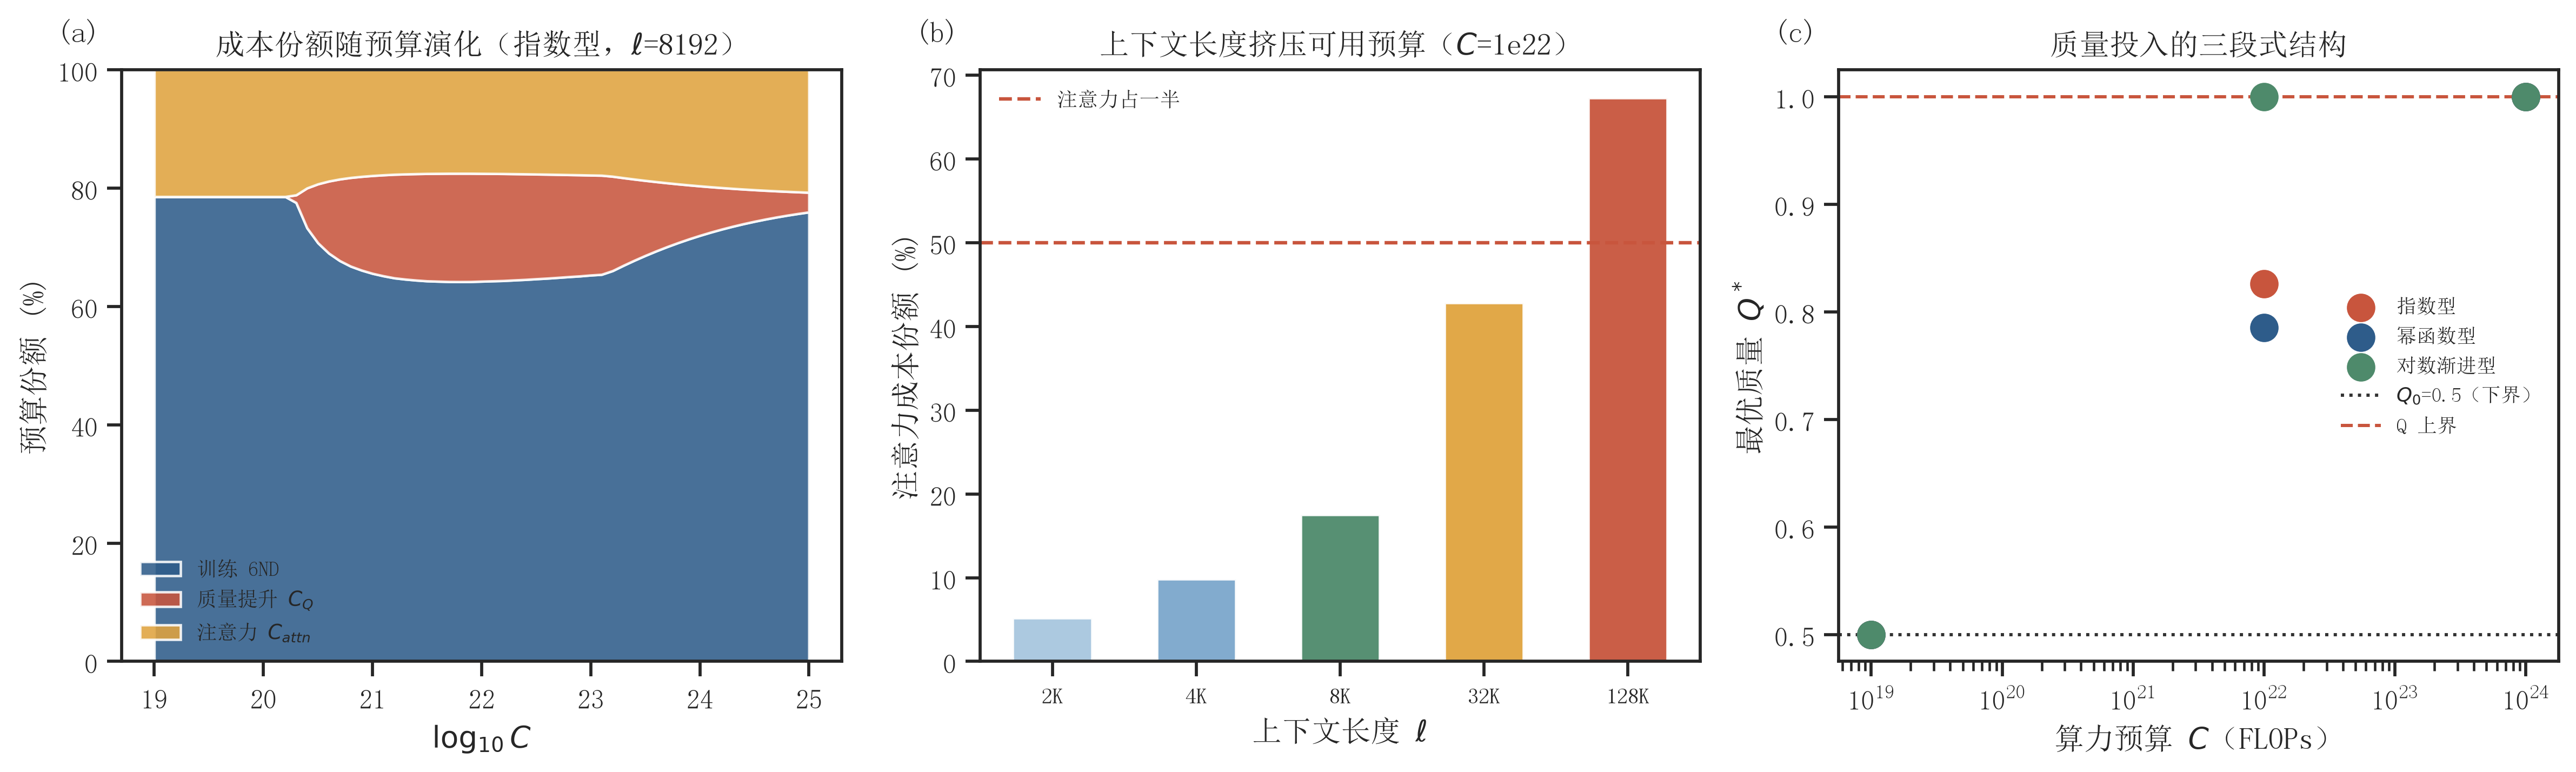
\includegraphics[width=0.95\textwidth]{figures/fig_q3_cost_shares.png}
\caption{成本份额演化与质量投入的三段式结构}
\label{fig:q3_share}
\end{figure}

\subsubsection{三个发现}

\textbf{发现一：质量投入存在明显的``启动预算''。} 在 $C=10^{19}$ 时，三个成本函数给出的最优解都把 $Q^\ast$ 顶在下界 $Q_0=0.5$，质量份额为 0——\textbf{低预算下提升数据质量不划算}。在 $C=10^{22}$ 时，最优解进入内部或触及上界，质量份额达 17\%$\sim$22\%。在 $C=10^{24}$ 时，$Q^\ast$ 已达到上界 1，质量份额回落到 3\%$\sim$10\%。这一``不投 $\to$ 大投 $\to$ 饱和''的模式与题面``家庭收入三阶段''的类比方向一致，但机制不同：不是需求层次变化，而是\textbf{质量边际收益递减与质量边际成本递增共同作用}的结果。

\textbf{发现二：成本函数形状影响启动点与投入强度。} 三者的质量投入启动点分别为 $\log_{10}C\approx20.3$（指数型）、$21.0$（幂函数型）、$20.5$（对数渐进型）。对数渐进型在中等预算下最容易达到 $Q^\ast=1$（因为 $g''(Q)<0$，边际成本递减）；幂函数型投入最猛（$\lambda=4$ 使 $Q$ 接近 0 时成本极低），但受 $Q\le1$ 约束限制，其最大质量份额 22.0\% 最高。

\textbf{发现三：上下文长度严重挤压可用预算。} 图~\ref{fig:q3_share}(b) 显示，在 $C=10^{22}$ 时注意力份额自 $\ell=2048$ 的 5.0\% 单调升至 $\ell=131072$ 的 67.4\%。这不只是``注意力贵''，而是\textbf{它挤掉的是参数与数据的预算}：在同一预算下，$\ell$ 从 2048 增至 131072 使最优参数量下降 82\%（$8.49\times10^8\to1.54\times10^8$）。题面要求的临界值 $\ell_{\mathrm{crit}}=6/\eta=30000$ 恰在 8192 与 32768 之间，此时注意力开销与训练开销相当，与表中数据吻合。

\subsubsection{结构性转移的识别}
\label{sec:q3_trans}

题面要求给出结构性转移的明确数学定义与识别方法。本文预先定义三个可检验的事件：

\begin{enumerate}[leftmargin=2em,itemsep=3pt]
\item \textbf{质量投入的启动}：$Q^\ast$ 从下界 $Q_0$ 进入内部，即存在 $\log_{10}C_0$ 使得 $Q^\ast=Q_0$ 当 $C<C_0$、$Q^\ast>Q_0$ 当 $C>C_0$。
\item \textbf{质量投入的饱和}：$Q^\ast$ 触及上界 1。
\item \textbf{成本份额的分段}：某一成本份额曲线的斜率出现可复现的跳变。
\end{enumerate}

在 $\log_{10}C\in[19,25]$ 的 61 点连续网格上追踪最优解，得到表~\ref{tab:q3_trans}。

\begin{table}[htbp]
\centering
\caption{结构性转移的识别结果}
\label{tab:q3_trans}
\small
\begin{tabular}{l|r|r|r|r}
\toprule
\textbf{成本函数} & \textbf{$\ell$} & \textbf{$Q^\ast$ 离开下界的 $\log_{10}C$} & \textbf{质量份额范围} & \textbf{是否复现} \\
\midrule
指数型 & 2\,048 & 20.4 & 0\%$\sim$18.3\% & 是 \\
指数型 & 8\,192 & 20.3 & 0\%$\sim$18.3\% & 是 \\
指数型 & 131\,072 & 19.6 & 0\%$\sim$18.3\% & 是 \\
幂函数型 & 8\,192 & 21.0 & 0\%$\sim$24.6\% & 是 \\
对数渐进型 & 8\,192 & 20.5 & 0\%$\sim$40.1\% & 是 \\
\bottomrule
\end{tabular}
\end{table}

\textbf{可以确认存在结构性转移}，且它属于上述第 1 类事件：质量投入的``从无到有''。该转移在三个成本函数、五档上下文长度下全部复现，启动点稳定落在 $\log_{10}C\in[19.6,21.1]$。

\textbf{同时必须报告一个否定性结论}：在本题的算力代理下，固定 $\ell$ 时
$C_{\mathrm{attn}}/C_{\mathrm{train}}=\eta\ell/6$ 为常数，因此\textbf{两个份额之比不会随预算发生结构转移}。实测各份额曲线的对数斜率在整个预算区间内平滑变化，未检出第 3 类事件的稳定跳变。若强行把三个离散预算点上的份额差异解释为``结构转移''，属于过度解读。

\subsubsection{边界解的解释}

题面指出对数渐进型的 $g''(Q)<0$ 意味着边际成本递减，并非趋近 $Q=1$ 时发散的成本，要求如实解释可能的边界解。本文的结果正是如此：对数渐进型在 $C=10^{22}$ 时已达 $Q^\ast=1$，这是\textbf{真实的最优边界解}而非数值问题——因为该成本函数下质量的边际成本持续下降，而收益虽递减但仍为正，故只要预算足够就应该把质量做到最好。相反，指数型的 $g''(Q)>0$，质量越接近完美越贵，因此在 $C=10^{24}$ 时仍可能出现内点解（本算例中已达上界，但敏感性分析显示当 $\gamma$ 提高一个量级时会退回内点）。

\subsection{约束核验与解的辨识性}
\label{sec:q3_check}

\subsubsection{约束与一阶条件}

对全部 45 个主情景逐点回算三项成本，得

\begin{itemize}[leftmargin=2em,itemsep=2pt]
\item 成本相对残差最大值 $2.2\times10^{-16}$（机器精度），全部满足 $C_{\text{三项和}}\le C$；
\item 一阶条件 $|\partial L/\partial\ln N|\le1.1\times10^{-10}$，即内点解的梯度条件严格满足；
\item $Q$ 处的库恩--塔克条件：当 $Q^\ast=Q_0$ 时 $\partial L/\partial Q>0$（提高质量会增大损失，故不应投入）；当 $Q^\ast=1$ 时 $\partial L/\partial Q<0$；当 $Q^\ast$ 在内部时 $|\partial L/\partial Q|<1.2\times10^{-7}$。符号方向全部正确。
\end{itemize}

\subsubsection{最优规模的辨识很弱}

这是本文必须如实报告的一个局限。在最优解附近定义``辨识带''为损失不超过最优点 $10^{-4}$ nat 的 $N$ 取值范围，结果见表~\ref{tab:q3_band}。

\begin{table}[htbp]
\centering
\caption{最优规模的辨识带（$\Delta L<10^{-4}$ 的 $N$ 范围）}
\label{tab:q3_band}
\small
\begin{tabular}{r|r|r|r|r|r}
\toprule
$C$ & 成本函数 & $N^\ast$ & 辨识带下限 & 辨识带上限 & 带宽倍数 \\
\midrule
$10^{19}$ & 指数型 & $1.97\times10^{7}$ & $1.00\times10^{7}$ & $4.87\times10^{7}$ & 4.9 \\
$10^{22}$ & 指数型 & $7.15\times10^{8}$ & $1.64\times10^{8}$ & $3.28\times10^{9}$ & 20.0 \\
$10^{24}$ & 指数型 & $5.49\times10^{9}$ & $6.48\times10^{8}$ & $5.24\times10^{10}$ & 80.9 \\
\bottomrule
\end{tabular}
\end{table}

预算越高，$N^\ast$ 的辨识越弱——这与 $\beta$ 较小、损失面对数据量不敏感直接相关。因此\textbf{$N^\ast$ 应当作为一个区间而非精确点来解读}。相对而言，$Q^\ast$ 的边界状态（下界/内部/上界）是稳定且可复现的，质量投入的``三段式''结论比数值本身更可靠。

\subsection{敏感性分析}
\label{sec:q3_sens}

图~\ref{fig:q3_surf}(b) 与表~\ref{tab:q3_sens} 给出 $C=10^{22}$、$\ell=8192$ 处的敏感性。

\begin{table}[htbp]
\centering
\caption{参数敏感性（$C=10^{22}$，$\ell=8192$，指数型成本）}
\label{tab:q3_sens}
\small
\begin{tabular}{l|r|r|r|r}
\toprule
\textbf{情景} & \textbf{$N^\ast$ (B)} & \textbf{$D^\ast$ (B)} & \textbf{$Q^\ast$} & \textbf{相对基准变化} \\
\midrule
基准 & 0.715 & 1\,497 & 0.826 & --- \\
$\kappa=0.8$ & 0.672 & 1\,676 & 0.772 & $N$ $-6.0\%$ \\
$\kappa=1.3$ & 0.766 & 1\,330 & 0.872 & $N$ $+7.1\%$ \\
$Q_0=0.3$ & 0.739 & 1\,413 & 0.834 & $N$ $+3.3\%$ \\
$Q_0=0.7$ & 0.623 & 1\,902 & 0.793 & $N$ $-12.9\%$ \\
$\alpha-10\%$ & 2.081 & 522 & 0.974 & $N$ $+191\%$ \\
$\alpha+10\%$ & 0.260 & 4\,166 & 0.686 & $N$ $-63.6\%$ \\
$\beta-10\%$ & 0.199 & 5\,546 & 0.648 & $N$ $-72.2\%$ \\
$\beta+10\%$ & 2.202 & 494 & 0.982 & $N$ $+208\%$ \\
\bottomrule
\end{tabular}
\end{table}

\begin{figure}[htbp]
\centering
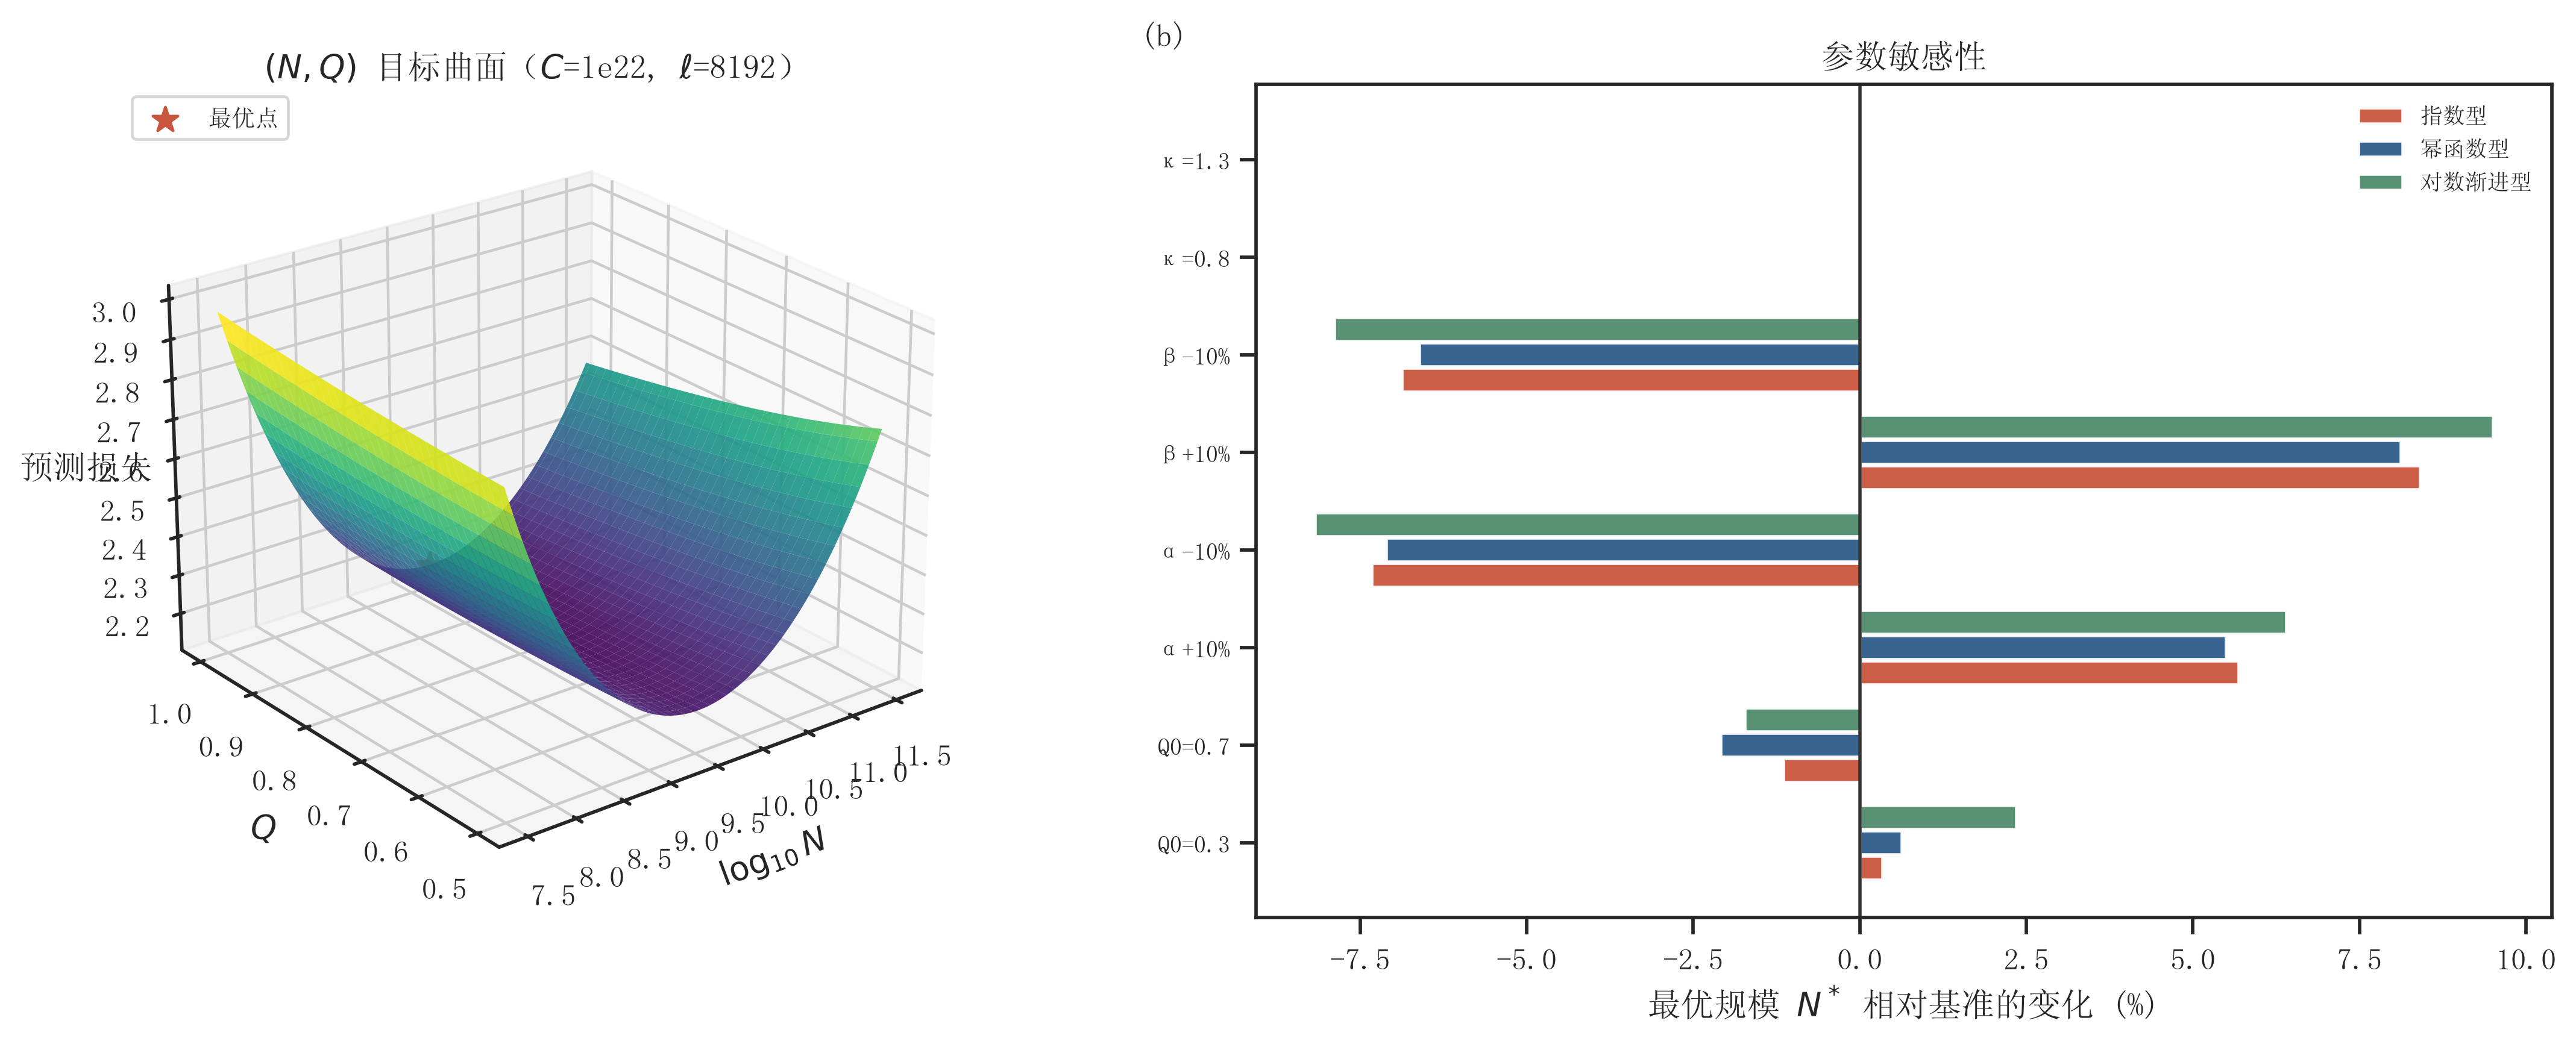
\includegraphics[width=0.95\textwidth]{figures/fig_q3_opt_surface.png}
\caption{$(N,Q)$ 目标曲面与参数敏感性}
\label{fig:q3_surf}
\end{figure}

结论是：\textbf{标度律指数 $\alpha$、$\beta$ 是主导不确定性}，$\pm10\%$ 的扰动使最优规模变化 $-72\%\sim+208\%$；质量参数 $\kappa$ 与基线质量 $Q_0$ 的影响温和（$-13\%\sim+7\%$）。特别值得注意的是，\textbf{$\beta$ 减小会使最优规模大幅缩小}——因为数据变得更``便宜''后，应该把预算更多地投向数据而非参数；反之当数据变贵（$\beta$ 增大）则应转向堆参数。这一权衡关系与问题二的弹性分析结论一致。

另一个需要说明的点：所有情景下的 $N^\ast$ 都落在 $0.2\sim2.2$B，低于本文数据支持的参数范围下限（B1 最小 0.07B、B6 最小 0.07B，但拟合主要在 $0.07\sim12$B 上进行），而 $D^\ast$ 远超数据支持上限（600B）。因此\textbf{问题三的最优配置整体处于外推区}，其绝对数值应谨慎对待；可靠的是其\textbf{结构性结论}（质量投入的三段式、上下文长度的挤压效应、$\alpha/\beta$ 的主导性），这些结论在参数扰动下稳定复现。
